Antes de proceder con la asignatura de Álgebra III, cuyo principal objetivo es dar solución a las ecuaciones polinómicas mediante el uso y estudio de los cuerpos finitos, recomendamos repasar en anteriores apuntes los siguientes conceptos:
\begin{itemize}
    \item En los apuntes de Álgebra I los conceptos de: anillo, subanillo, homomorfismo de anillos e ideal; así como la forma en la que se estudiaba que un polinomio era irreducible.
    \item En los apuntes de Álgebra II los conceptos de: grupo, subgrupo, homomorfismo de grupos y monoide.
\end{itemize}
Una vez repasados dichos conceptos, estamos en condiciones de comenzar la asignatura.

\chapter{Extensiones de cuerpos y raíces de polinomios}
\noindent
Comenzamos definiendo el objeto de estudio protagonista a lo largo de esta asignatura: los cuerpos, llamados a veces campos, del inglés \textit{fields}.

\begin{notacion}
    Aunque las dos operaciones de los anillos (y también de los cuerpos) no tengan por qué ser una suma y una multiplicación, optaremos por dichas notaciones, junto con las notaciones de ``cero'' para el elemento neutro de la operación ``suma'' y de ``uno'' para el elemento neutro de la operación ``producto''; por ser familiares a los anillos a los que estamos acostumbrados. De esta forma, para nosotros un anillo será una tupla $(A,+,0,\cdot,1)$, a la que podremos referirnos simplemente por $A$ cuando las dos operaciones y elementos neutros estén claros por el contexto.
\end{notacion}

\begin{definicion}[Cuerpo]
    Un cuerpo es un anillo $A$ en el que $A\setminus \{0\}$ es un grupo.
\end{definicion}

Observemos que estamos suponiendo implícitamente que el anillo $\{0\}$ jamás puede ser un cuerpo.

\begin{ejemplo}
    Algunos ejemplos de los cuerpos más famosos son:
    \begin{itemize}
        \item $\mathbb{Q}$.
        \item $\mathbb{R}$.
        \item $\mathbb{C}$.
        \item $\mathbb{Z}_p$ con $p$ primo.
    \end{itemize}
\end{ejemplo}

\noindent
Con el objetivo de definir de forma totalmente rigurosa lo que es la característica de un anillo (concepto que puede que se haya mencionado ya en cursos anteriores), nos es necesaria la siguiente proposición:
\begin{prop}
    Sea $A$ un anillo, existe un único homomorfismo de anillos
    \begin{equation*}
        \chi:\mathbb{Z}\to A
    \end{equation*}
    Además, $Im\chi$ es el menor subanillo contenido en $A$.
    \begin{proof}
        Sean $\chi,\varphi:\mathbb{Z}\to A$ dos homomorfismos de anillos, demostremos por inducción que $\chi(k) = \varphi(k)$ para todo $k\in \mathbb{Z}$:
        \begin{description}
            \item [Para $k=1$.] Como $\chi$ y $\varphi$ son homomorfismos de anillos, estos cumplen 
                \begin{equation*}
                    \chi(1) = 1 = \varphi(1)
                \end{equation*}
            \item [Para $k=0$.] De manera análoga, $\chi(0) = 0 = \varphi(0)$.
            \item [Supuesto para todo $s\leq k$], vemos que:
                \begin{gather*}
                    \chi(k+1) = \chi(k) + \chi(1) = \varphi(k) + \varphi(1) = \varphi(k+1) \\
                    \chi(-(k+1)) = -\chi(k+1) = -\varphi(k+1) = \varphi(-(k+1))
                \end{gather*}
        \end{description}
        Acabamos de probar que $\chi = \varphi$, por lo que en caso de existir solo existe un único homomorfismo $\chi:\mathbb{Z}\to A$. Este se puede calcular exigiendo $\chi(1)= 1$.\\

        \noindent
        Ahora, para ver que $Im\chi$ es el menor subanillo contenido en $A$, vimos ya en Álgebra I que $Im\chi$ es un subanillo de $A$. Para ver que es el menor, sea $S\subseteq A$ otro subanillo de $A$, como subanillo de $A$ que es ha de contener al 1, al 0 y ser cerrado para sumas y opuestos, luego ha de contener también a $n\cdot 1$ y $-(n\cdot 1)$, para todo $n\in \mathbb{N}$. Sin embargo, tenemos que:
        \begin{equation*}
            Im\chi = \{\chi(n) : n\in \mathbb{Z}\} = \{0\}\cup \left\{\sum_{k=1}^{n}\chi(1) : n\in \mathbb{N}\right\} \cup \left\{\sum_{k=1}^{n}\chi(-1) : n\in \mathbb{N}\right\}
        \end{equation*}
         Por lo que $Im\chi \subseteq S$.
    \end{proof}
\end{prop}

\begin{definicion}[Característica de un anillo]
    Sea $A$ un anillo, sabemos por la Proposición anterior que existe un único homomorfismo de anillos 
    \begin{equation*}
        \chi:\mathbb{Z}\to A
    \end{equation*}
    En dicho caso, sabemos de Álgebra I que $\ker\chi$ es un ideal en $\mathbb{Z}$, y como todos los ideales de $\mathbb{Z}$ son principales (por ser $\mathbb{Z}$ un Dominio Euclídeo), sabemos que $\exists n\in \mathbb{N}$ de forma que $\ker\chi = n\mathbb{Z}$. Dicho número $n$ recibe el nombre de ``característica de $A$'' (aunque varios números cumplan esta definición, suele tomarse el más pequeño de ellos que sea positivo, en caso de no ser el ideal trivial).
\end{definicion}

\begin{prop}
    La característica de un cuerpo ha de ser un número primo o cero.
    \begin{proof}
        Supongamos que $A$ es un cuerpo de característica $n\neq 0$, por lo que:
        \begin{equation*}
            \sum_{k=1}^{n}1 = n\cdot 1 = 0
        \end{equation*}
        Por reducción al absurdo, supongamos que $n$ no es primo, con lo que puedo encontrar un primo $p$ y $m\neq 0$ de forma que:
        \begin{equation*}
            0 = n\cdot 1 = p\cdot m
        \end{equation*}
        Como $0\neq m \in A$, existe $m^{-1}\in A$, que puede multiplicarse a ambos lados de la igualdad, obteniendo que $p = 0$, contradicción, por lo que $n$ ha de ser primo.
    \end{proof}
\end{prop}

\begin{definicion}[Subcuerpos y extensiones de cuerpos]
    Si $K$ es un cuerpo, un subcuerpo de $K$ es un subanillo $F$ de $K$ tal que $F$ es un cuerpo. En dicho caso, diremos que $K$ es una extensión del cuerpo $F$, y se podrá notar por:
    \begin{equation*}
        F\leq K
    \end{equation*}
\end{definicion}

\section{Subcuerpos primos}
\noindent
Es fácil ver (hágase) que las intersecciones arbitrarias de cuerpos siguen siendo cuerpos, propiedad que justifica el concepto que vamos a introducir.

\begin{definicion}[Subcuerpo generado por un conjunto]
    Sea $K$ un cuerpo y $S\subseteq K$, si consideramos:
    \begin{equation*}
        \Gamma = \{F\subseteq K : F\leq K \text{\ y\ } S\subseteq F\}
    \end{equation*}
    es decir, el conjunto de todos los subcuerpos de $K$ que contienen a $S$, definimos el subcuerpo de $K$ generado por $S$ como el subcuerpo:
    \begin{equation*}
        \bigcap_{F\in \Gamma} F
    \end{equation*}
    Que se caracteriza por ser el menor subcuerpo de $K$ que contiene a $S$.
\end{definicion}

\begin{definicion}[Subcuerpo primo de un cuerpo]
    Si dado un cuerpo $K$ pensamos en el subcuerpo generado por el conjunto vacío obtenemos el ``subcuerpo primo de $K$'', que viene dado por:
    \begin{equation*}
        \bigcap_{F\in \Gamma} F
    \end{equation*}
    donde $\Gamma = \{F\subseteq K : F\leq K\}$. Este es el menor subcuerpo de $K$.
\end{definicion}

\begin{prop}
    Sea $K$ un cuerpo de característica $p$, entonces el subcuerpo primo de $K$ es isomorfo a:
    \begin{itemize}
        \item $\mathbb{Z}_p$ si $p>0$.
        \item $\mathbb{Q}$ si $p = 0$.
    \end{itemize}
    \begin{proof}
        Si consideramos el único homomorfismo $\chi:\mathbb{Z}\to K$, tenemos que $Im\chi$ es el menor subanillo de $K$, por lo que estará contenido (hágase) en el subcuerpo primo de $K$, que denotaremos por $\Pi$; es decir, $Im\chi \subseteq \Pi$. Aplicando el Primer Teorema de Isomofría sobre $\chi$ obtenemos que:
        \begin{equation*}
            \dfrac{\mathbb{Z}}{p\mathbb{Z}} = \dfrac{\mathbb{Z}}{\ker\chi} \cong Im\chi 
        \end{equation*}
        \begin{description}
            \item [Si $p>0$] tendremos (vimos anteriormente que $p$ debe ser primo):
                \begin{equation*}
                    \mathbb{Z}_p = \dfrac{\mathbb{Z}}{p\mathbb{Z}} \cong Im\chi
                \end{equation*}
                Por lo que $Im\chi$ es un subcuerpo de $K$, y como $\Pi$ es el menor subcuerpo de $K$, tenemos que $\Pi\subseteq Im\chi$, lo que nos da la igualdad $\Pi = Im\chi \cong \mathbb{Z}_p$.
            \item [Si $p=0$] tendremos entonces $\mathbb{Z}\cong Im\chi$, por lo que los cuerpos de fracciones de $\mathbb{Z}$ y de $Im\chi$ (a quien denotaremos por $Q$) han de ser isomorfos:
                \begin{equation*}
                    \mathbb{Q}\cong Q
                \end{equation*}
                Como teníamos que $Im\chi \subseteq \Pi$, podemos calcular $Q$ dentro\footnote{Si $A\subseteq B$ como subanillo, entonces el cuerpo de fracciones de $A$ está dentro del cuerpo de fracciones de $B$, pero si $B$ es un cuerpo, coincide con su cuerpo de fracciones.} de $\Pi$, obteniendo que $Q\subseteq \Pi$, pero como $\Pi$ es el menor subcuerpo de $K$, tendremos $\Pi\subseteq Q$, lo que nos da la igualdad $\Pi = Q \cong \mathbb{Q}$.\qedhere
        \end{description}
    \end{proof}
\end{prop}

\begin{observacion}
    Si $F\leq K$ extensión, entonces $K$ es un espacio vectorial sobre $F$.
\end{observacion}

\begin{definicion}
    Si $F\leq K$ es una extensión, la dimensión de $K$ sobre $F$ como espacio vectorial recibe el nombre de ``grado de la extensión $F\leq K$'', denotado por: 
    \begin{equation*}
        [K:F]
    \end{equation*}
    Si $[K:F]$ es un número finito, decimos que $F\leq K$ \underline{es (una extensión) finita}. En caso contrario, diremos que es una extensión infinita, denotado por $[K:F] = \infty$.
\end{definicion}

\begin{ejemplo}
    Como ejemplos a destacar:
    \begin{itemize}
        \item $\mathbb{R}\leq \mathbb{C}$ tiene grado de extensión $[\mathbb{C}:\mathbb{R}] = 2$.
        \item Si $[\mathbb{R}:\mathbb{Q}] = n$, entonces tendríamos que $\mathbb{R}\cong \mathbb{Q}^n$ como subespacios vectoriales, por lo que $\mathbb{R}$ no sería numerable. Por tanto, podemos decir que $[\mathbb{R}:\mathbb{Q}]=\infty$.
    \end{itemize}
\end{ejemplo}

\begin{ejercicio}
    Demostrar que el cardinal de un cuerpo finito es de la forma $p^n$, con $p$ primo y $n\geq 1$.\\

    \noindent
    Sea $K$ un cuerpo finito, este no podrá tener característica cero, por lo que su característica será un primo $p$ de forma que su cuerpo primo será isomorfo a $\mathbb{Z}_p$. De esta forma, $K$ será un espacio vectorial sobre un cuerpo isomorfo a $\mathbb{Z}_p$, con cierto grado de extensión $n\in \mathbb{N}\setminus \{0\}$, por lo que \underline{como espacio vectorial} será isomorfo a:
    \begin{equation*}
        \underbrace{\mathbb{Z}_p\times \ldots \times \mathbb{Z}_p}_{n\text{ veces }}
    \end{equation*}
    Luego $K$ ha de tener cardinal $p^n$.
\end{ejercicio}

\noindent
Haremos próximamente una clasificacion de cuerpos finitos, en la que cada primo y natural no nulo nos definan un único cuerpo de cardinal $p^n$.

\section{Extensiones de cuerpos y elementos algebraicos}

\begin{definicion}[Extensión generada por un subconjunto]
    Sea $F\leq K$ extensión, $S\subseteq K$, definimos la ``extensión de $F$ generada por $S$'' como el menor subcuerpo de $K$ que contiene a $F\cup S$, denotado por $F(S)$.
    \begin{itemize}
        \item Si $S = \{s_1,\ldots,s_t\}$, simplificaremos la notación y escribiremos $F(s_1,\ldots,s_t)$.
        \item Si $K = F(\alpha_1, \ldots, \alpha_t)$ para ciertos elementos $\alpha_1, \ldots, \alpha_t\in K$, diremos entonces que $F\leq K$ \underline{es una extensión finitamente generada}\footnote{No confundir una extensión finitamente generada con una extensión finita de cuerpos.}.
    \end{itemize}
\end{definicion}

\begin{ejemplo}
    $\mathbb{Q}(\sqrt{2})$ es el menor subcuerpo de $\mathbb{R}$ que contiene a $\sqrt{2}$, y viene dado por:
    \begin{equation*}
        \mathbb{Q}(\sqrt{2}) = \left\{a+b\sqrt{2} : a,b\in \mathbb{Q}\right\}
    \end{equation*}
    \begin{proof}
        Veámoslo:
        \begin{description}
            \item [$\supseteq)$] Sean $a,b\in \mathbb{Q}$, tenemos que $a,b,\sqrt{2}\in \mathbb{Q}(\sqrt{2})$, por lo que $a+b\sqrt{2}\in \mathbb{Q}(\sqrt{2})$.
            \item [$\subseteq)$] Si demostramos que $\{a+b\sqrt{2}:a,b\in \mathbb{Q}\}$ es un cuerpo, entonces tenemos esta inclusión, ya que $\mathbb{Q}(\sqrt{2})$ es el menor subcuerpo de $\mathbb{R}$ que contiene a $\sqrt{2}$. Es evidente que dicho conjunto es un anillo. Para ver que es un cuerpo, dado $\alpha=a+b\sqrt{2}$, buscamos calcular un elemento inverso al mismo que sea de la misma forma. Sea:
                \begin{equation*}
                \beta = \dfrac{a}{a^2-2b^2} - \dfrac{b\sqrt{2}}{a^2-2b^2} = \dfrac{a-b\sqrt{2}}{a^2-2b^2} \in \{a+b\sqrt{2}:a,b\in \mathbb{Q}\}
                \end{equation*}
                Observamos que:
                \begin{equation*}
                    \alpha \beta = \left(a+b\sqrt{2}\right) \dfrac{a-b\sqrt{2}}{a^2-2b^2} = \dfrac{\left(a+b\sqrt{2}\right)\left(a-b\sqrt{2}\right)}{\left(a+b\sqrt{2}\right)\left(a-b\sqrt{2}\right)} = 1
                \end{equation*}
                Por lo que dicho conjunto es un cuerpo, al tener todo elemento un inverso.
        \end{description}
    \end{proof}
    Observamos que tenemos $\left[\mathbb{Q}(\sqrt{2}): \mathbb{Q}\right] = 2$. Debemos tener en cuenta que aunque este resultado puede tener otro más general como que:
    \begin{equation*}
        \mathbb{Q}(\sqrt{n}) = \{a+b\sqrt{n}:a,b\in \mathbb{Q}\} \qquad \sqrt{n}\notin \mathbb{Q}
    \end{equation*}
    En general, esta no es la definición del menor subcuerpo generado por cierto conjunto.
\end{ejemplo}

\begin{definicion}[Cuerpo de descomposición]
    Sea $K$ un cuerpo, $f\in K[x]$ y $K\leq E$ extensión de cuerpos tal que $f$ se descompone completamente en $E[x]$ como producto de polinomios lineales (es decir, de grado 1) y $E=K(\alpha_1,\ldots,\alpha_t)$ con $\alpha_1,\ldots,\alpha_t\in E$ las raíces de $f$, entonces diremos que $E$ es un cuerpo de descomposición (o de escisión) de $f$ sobre $K$.
\end{definicion}

% De algebra I, solo los polinomios de grado 2 o 3 sin raices son irreducibles, para mayor grado ser irreducible es algo más

\begin{ejemplo}
    Veamos varios ejemplos de cuerpos de descomposición de polinomios:
    \begin{itemize}
        \item Si consideramos $x^2+1\in \mathbb{R}[x]$, como $\mathbb{R}\leq \mathbb{C}$ y se cumple que $\mathbb{C} = \mathbb{R}(i,-i)$, tenemos que $\mathbb{C}$ es un cuerpo de descomposición de $x^2+1$.
        \item Por ejemplo, si $x^2+1\in \mathbb{Q}[x]$, un cuerpo de descomposición en este caso es $\mathbb{Q}(i)$, ya que $\mathbb{Q}\leq \mathbb{Q}(i)$ y $\mathbb{Q}(i) = \mathbb{Q}(i,-i)$.
    \end{itemize}
\end{ejemplo}

\begin{observacion}
    Si $f\in \mathbb{Q}[x]$ y tomo\footnote{Fundamentado por el Teorema Fundalmental del Álgebra.} todas sus raíces en $\mathbb{C}$, digamos $\alpha_1,\ldots,\alpha_t$, entonces un cuerpo de descomposición de $f$ es $\mathbb{Q}(\alpha_1,\ldots,\alpha_t)$
\end{observacion}

\begin{ejemplo}
    Si tomamos $x^2-2\in \mathbb{Q}[x]$, entonces un cuerpo de descomposición es $\mathbb{Q}(\sqrt{2})$.
\end{ejemplo}

\begin{ejercicio}
    Si tenemos $F\leq K$ extensión de cuerpos y $S,T\subseteq K$, demostrar que:
    \begin{equation*}
        F(S\cup T) = F(S)(T)
    \end{equation*}
    \begin{proof}
        Veámoslo por doble inclusión:
        \begin{description}
            \item [$\subseteq )$] $F(S\cup T)$ es por definición el menor subucerpo de $K$ que contiene a $F\cup S\cup T$, por lo que para ver esta inclusión hemos de ver que $F(S)(T)$ es un cuerpo que contiene a $F\cup S\cup T$. Para ello, $F(S)(T)$ es por definición el menor subcuerpo de $K$ que contiene a $F(S)\cup T$, y $F(S)$ es a su vez el menor subcuerpo de $K$ que contiene a $F\cup S$. Por tanto, $F(S)(T)$ es un cuerpo que contiene a $F\cup S\cup T$, de donde $F(S\cup T)\subseteq F(S)(T)$.
            \item [$\supseteq )$] El menor subcuerpo de $K$ que contiene a $F\cup S\cup T$ ha de contener al menor subcuerpo de $K$ que contiene a $F\cup S$, por lo que $F(S\cup T)\supseteq F(S)$. Como ahora tenemos que $F(S),T\subseteq F(S\cup T)$, tenemos por tanto que el menor subcuerpo de $K$ que contiene a $F(S)\cup T$ está contenido en $F(S\cup T)$, es decir, $F(S)(T)\subseteq (S\cup T)$.
        \end{description}
    \end{proof}
\end{ejercicio}

\begin{ejemplo}
    Si tomamos $f=x^3-2\in \mathbb{Q}[x]$, este polinomios tiene 3 raíces distintas, ya que su polinomio derivado\footnote{Recordamos que si $\alpha$ es una raíz múltiple de $f$, entonces $\alpha$ es una raíz de $f'$.} tiene como raíces el cero, que no es raíz de $f$. Las raíces de $f$ son $\sqrt[3]{2}$ y el resto son dos raíces complejas, que se calculan usando las raíces terciarias de la unidad:
    \begin{equation*}
        \omega = e^{\frac{2\pi i}{3}} = \cos\left(\frac{2\pi}{3}\right) + i\sen\left(\frac{2\pi}{3}\right) = \dfrac{-1}{2} + i \dfrac{\sqrt{3}}{2}
    \end{equation*}
    Por lo que $\omega^3 = 1$, de donde ${\left(\sqrt[3]{2}\omega\right)}^{3} = 2$. Así que un cuerpo de descomposición de $f$ es $\mathbb{Q}\left(\sqrt[3]{2}, \omega\sqrt[3]{2}, \omega^2\sqrt[3]{2}\right)$, que es igual a $\mathbb{Q}\left(\sqrt[3]{2},\omega\right)$:
    \begin{proof}
        Por doble inclusión:
        \begin{description}
            \item [$\subseteq )$] Como $\mathbb{Q}\left(\sqrt[3]{2}, \omega\right)$ es un cuerpo que contiene a $\omega$ y a $\sqrt[3]{2}$, este ha de contener también a:
                \begin{equation*}
                    \sqrt[3]{2}, \quad \omega\sqrt[3]{2}, \quad \omega^2 \sqrt[3]{2}
                \end{equation*}
                Por lo que el menor cuerpo que contiene a todos estos ha de estar contenido en $\mathbb{Q}\left(\sqrt[3]{2}, \omega\right)$.
            \item [$\supseteq )$] De forma análoga, como $\mathbb{Q}\left(\sqrt[3]{2}, \omega\sqrt[3]{2}, \omega^2\sqrt[3]{2}\right)$ es un cuerpo que contiene a $\sqrt[3]{2}$ y a $\omega$, ya que:
                \begin{equation*}
                    \omega = \dfrac{\omega \sqrt[3]{2}}{\sqrt[3]{2}} \in \mathbb{Q}\left(\sqrt[3]{2}, \omega\sqrt[3]{2}, \omega^2\sqrt[3]{2}\right)
                \end{equation*}
                Por tanto, el menor cuerpo que contiene a $\omega$ y $\sqrt[3]{2}$ ha de estar contenido en $\mathbb{Q}\left(\sqrt[3]{2}, \omega\sqrt[3]{2}, \omega^2\sqrt[3]{2}\right)$.
        \end{description}
    \end{proof}
\end{ejemplo}

\noindent
Nos preguntamos ahora por un cuerpo de descomposición de $x^2+x+1\in \mathbb{Z}_2[x]$. Todavía no podemos dar respuesta a esta pregunta, por lo que necesitamos una noción más sofisticada de cuerpos de descomposición, a la que llegaremos desarrollando esta teoría.

\begin{ejemplo}
    Tomamos $f=x^n-1\in \mathbb{Q}[x]$ con $n\geq 1$ y nos preguntamos sobre un cuerpo de descomposición de dicho polinomio, que tiene $n$ raíces, y:
    \begin{equation*}
        f' = nx^{n-1}
    \end{equation*}
    Por lo que no comparte raíces con $f'$, luego tiene $n$ raíces distintas, todas ellas de multiplicidad 1, que son:
    \begin{equation*}
        \left\{{\left(e^{\frac{2\pi i}{n}}\right)}^{k}:k\in \{0,\ldots,n-1\}\right\}
    \end{equation*}
    Que es un subgrupo cíclico de orden $n$ de $\mathbb{C}\setminus\{0\}$, generado por $e^{\frac{2\pi i}{n}}$. Cada uno de sus generadores se llama \underline{raíz $n-$ésima compleja primitiva de la unidad}.\\

    \noindent
    Un cuerpo de descomposición de $x^n-1\in \mathbb{Q}[x]$ es $\mathbb{Q}(\eta)$, donde $\eta$ es una raíz $n-$ésima compleja primitiva de la unidad.
\end{ejemplo}

\subsection{Elementos algebraicos}
\noindent
Algo que tienen en común todos los números complejos que aparecían en los ejemplos anteriores es que todos ellos son algebraicos sobre $\mathbb{Q}$:

\begin{definicion}[Elemento algebraico]
    Sea $F\leq K$ extensión y $\alpha\in K$, diremos que $\alpha$ es algebraico \red{sobre} $F$ si $f(\alpha)=0$ para algún $f\in F[x]\setminus\{0\}$. En caso contrario, diremos que $\alpha$ es \underline{trascendente} sobre $F$.
\end{definicion}

\begin{prop}\label{prop:pol_irreducible}
    Sean $F\leq K$ extensión, $\alpha\in K$ algebraico sobre $F$. Existe un único polinomio mónico\footnote{El coeficiente líder es 1.} irreducible $f\in F[x]$ tal que $f(\alpha)=0$. Además, se tiene un isomorfismo de cuerpos $F(\alpha)\cong \dfrac{F[x]}{\langle f \rangle }$, donde $\langle f \rangle $ denota el ideal principal generado por $f$:
    \begin{equation*}
        \langle f \rangle  = \{gf : g\in F[x]\}
    \end{equation*}
    Y además, $\{1,\alpha, \ldots, \alpha^{deg f - 1}\}$ es una $F-$base de $F(\alpha)$. Así, $[F(\alpha): F] = degf$.
    \begin{proof} 
        Definimos la aplicación $e_\alpha:F[x]\to K$ por:
        \begin{equation*}
            e_\alpha(g) = g(\alpha) \qquad \forall g\in F[x]
        \end{equation*}
        que es un homomorfismo de anillos (compruébese). Por tanto, su núcleo $\ker e_\alpha$ es un ideal de $F[x]$. Como $F$ es un cuerpo, $F[x]$ es un Dominio Euclídeo, luego todo ideal es principal. Sea $f\in F[x]$ el generador mónico de $\ker e_{\alpha}$, sabemos que es el polinomio de menor grado contenido en $\ker e_{\alpha}$. Veamos que $f$ cumple con las condiciones descritas en el enunciado:
        \begin{itemize}
            \item Por la definición de $f$ tenemos que $f\in \ker e_\alpha$, luego:
                \begin{equation*}
                    0 = e_\alpha(f) = f(\alpha)
                \end{equation*}
            \item Por el Primer Teorema de Isomorfía, $e_{\alpha}$ induce un isomorfismo de anillos:
                \begin{equation*}
                    Im e_\alpha \cong \dfrac{F[x]}{\ker e_\alpha} = \dfrac{F[x]}{\langle f \rangle }
                \end{equation*}
                Donde $Im e_{\alpha}$ será un subanillo de $K$, que es un dominio de integridad por ser un cuerpo, luego $Im e_{\alpha}$ también es un dominio de integridad, de donde $\frac{F[x]}{\langle f \rangle }$ es un dominio de integridad también, luego por un teorema visto en Álgebra I deducimos que $f$ tiene que ser irreducible.
            \item Para ver la unicidad, si tomamos $h\in F[x]$ un polinomio mónico tal que $h(\alpha)=0$, entonces $h\in \ker e_\alpha = \langle f \rangle $, por lo que $\langle h \rangle \subseteq \langle f \rangle $. Como $h$ es irreducible, tenemos que $\langle h \rangle $ es un ideal maximal, de donde $\langle h \rangle  = \langle f \rangle $. Por tanto, existe $\lm\in F$ de forma que $h=\lm f$, pero como ambos son polinomios mónicos, ha de ser $\lm = 1$, luego $h = f$.
            \item Para ver el isomorfismo, como $\frac{F[x]}{\langle f \rangle }$ es un dominio de integridad, un Teorema de Álgebra I nos decía que entonces $\frac{F[x]}{\langle f \rangle }$ era un cuerpo, de donde el isomorfismo
                \begin{equation*}
                    Im e_\alpha \cong \dfrac{F[x]}{\langle f \rangle }
                \end{equation*}
                nos dice que $Im e_\alpha$ es un cuerpo, contenido en $K$: $Im e_\alpha \leq K$.

                Sea $a\in F$, podemos ver $a$ dentro de $F[x]$ como el polinomio constantemente igual a $a$, por lo que $e_\alpha(a) = a$, de donde $a\in Im e_\alpha$, luego $F\leq Im e_\alpha$.

                Si consideramos ahora el polinomio identidad $h=x\in F[x]$, tenemos que: $e_\alpha(h) = h(\alpha) = \alpha$, por lo que $\alpha\in Im e_\alpha$.

                En definitiva, $Im e_\alpha$ es un cuerpo que contiene a $F\cup \{\alpha\}$, por lo que por definición de $F(\alpha)$ tiene que ser $F(\alpha) \subseteq Im e_\alpha$. Para la otra inclusión, si cogemos un elemento de $Im e_\alpha$, este será de la forma $g(\alpha)$ para cierto $g\in F[x]$, que tendrá la forma:
                \begin{equation*}
                    g(x) = \sum_{i=1}^{n} g_i x^i\qquad g_i \in F
                \end{equation*}
                de donde:
                \begin{equation*}
                    g(\alpha) = \sum_{i=1}^{n} g_i \alpha^i
                \end{equation*}
                Con $g_i \in F$ y $\alpha \in F(\alpha)$, de donde $g(\alpha) \in F(\alpha)$, lo que nos da la inclusión $Im e_\alpha\subseteq F(\alpha)$ que nos faltaba. En definitiva:
                \begin{equation*}
                    F(\alpha) = Im e_\alpha \cong \dfrac{F[x]}{\langle f \rangle }
                \end{equation*}
            \item Para ver que $\cc{B}=\left\{1,\alpha,\ldots, \alpha^{degf-1}\right\}$ es una $F-$base de $F(\alpha)$, primero vamos a tratar de buscar una base en $\frac{F[x]}{\langle f \rangle }$ cuya imagen por el isomorfismo con $F(\alpha)$ sea la base buscada. Para ello, sea $g+\langle f \rangle \in \frac{F[x]}{\langle f \rangle }$, si $deg g \geq deg f$, entonces podemos encontrar $q,r\in F[x]$ de forma que:
                \begin{equation*}
                    g = fq + r \qquad \text{con} \qquad degr < degf
                \end{equation*}
                En dicho caso, tenemos que $g+\langle f \rangle = r+ \langle f \rangle $. Por tanto, cualquier elemento $g+\langle f \rangle $ de $\frac{F[x]}{\langle f \rangle }$ puede escribirse como:
                \begin{equation*}
                    g(x) = \sum_{i=1}^{degf-1} f_ix^i \qquad f_i \in F \quad \forall i \in \{1,\ldots,degf-1\}
                \end{equation*}
                Luego $B=\{1+\langle f \rangle,x+\langle f \rangle, \ldots, x^{degf-1}+\langle f \rangle  \}$ es un sistema de generadores de $\frac{F[x]}{\langle f \rangle }$, que además es una base por ser sus elementos linealmente independientes. El isomorfismo 
                \begin{equation*}
                    \dfrac{F[x]}{\langle f \rangle }\cong Im e_\alpha  = F(\alpha)  
                \end{equation*}
                viene dado por (a partir del Primer Teorema de Isomorfia) la correspondencia $g+\langle f \rangle \mapsto g(\alpha)$. Este es $F-$lineal, por lo que transforma la base $B$ en el conjunto $\cc{B}$. Como los isomorfismos lineales transforman bases en bases (visto en Geometría I), tenemos que $\cc{B}$ es una $F-$base de $F(\alpha)$.
        \end{itemize}
    \end{proof}
\end{prop}
% Un anillo cociente es un cuerpo <=> el polinomio f es irreducible

\begin{definicion}[Polinomio irreducible]
    En las condiciones de la Proposición anterior, dicho único polinomio $f$ recibe el nombre ``polinomio irreducible (o mínimo) de $\alpha$ sobre $F$'', y lo notaremos por $Irr(\alpha,F)$.

    \noindent
    Observemos que este cumple $[F(\alpha):F] = deg Irr(\alpha,F)$. A dicho grado lo llamaremos a veces \underline{grado de $\alpha$ sobre $F$}.
\end{definicion}

\noindent
La notación de mínimo se debe por cómo se ha obtenido $f$ en la demostración anterior: se ha obtenido como un generador de $\ker e_\alpha$, y en un cuerpo los generadores de los ideales se escogen tomando el polinomio de menor grado. Al ser mónico, tenemos garantizada su unicidad, por lo que es el polinomio de grado más pequeño del que $\alpha$ es raíz.

\begin{observacion}
    Todo otro polinomio $g\in F[x]$ con $g(\alpha)=0$ satisface que $g = hIrr(\alpha,F)$.
\end{observacion}

\begin{ejemplo}
    Veamos ejemplos de esta última definición:
    \begin{itemize}
        \item $Irr(i,\mathbb{Q}) = x^2+1 \in \mathbb{Q}[x]$, luego $\{1,i\}$ es una $\mathbb{Q}-$base de $\mathbb{Q}(i)$.
        \item $Irr(\sqrt{2}, \mathbb{Q}) = x^2-2 \in \mathbb{Q}[x]$.
        \item $Irr\left(e^{\frac{2\pi i}{3}}, \mathbb{Q}\right)$. Podríamos pensar primero en el polinomio $x^3-1$, pero este no es irreducible, ya que 1 es una raíz suya:
            \begin{equation*}
                x^3-1 = (x-1)\left(x^2+x+1\right)
            \end{equation*}
            Ahora, tenemos que $x^2+x+1$ es un polinomio del que $e^{\frac{2\pi i}{3}}$ es raíz, y además es un polinomio irreducible, ya que es de grado 2 y no tiene raíces en $\mathbb{Q}$, por lo que $Irr\left(e^{\frac{2\pi i}{3}}, \mathbb{Q}\right) = x^2+x+1$.

            Una $\mathbb{Q}-$base de $\mathbb{Q}\left(e^{\frac{2\pi i}{3}}\right)$ es $\left\{1,e^{\frac{2\pi i}{3}}\right\}$, luego:
            \begin{equation*}
                \left[\mathbb{Q}\left(e^{\frac{2\pi i}{3}}\right):\mathbb{Q}\right] = 2
            \end{equation*}
    \end{itemize}
\end{ejemplo}

\begin{ejercicio}
    Sea $F\leq K$ extensión y $\alpha\in K$ de grado 2 sobre $F$. Demostrar que $F(\alpha)$ es un cuerpo de descomposición de $Irr(\alpha,F)$.\\

    \noindent
    Si $\alpha$ es de grado 2 sobre $F$, entonces tenemos que $[F(\alpha):F] = 2 = deg~Irr(\alpha,F)$, por lo que tenemos que $\exists a,b\in F$ de forma que:
    \begin{equation*}
        Irr(\alpha,F) = x^2+ax+b
    \end{equation*}
    puesto que sabemos que $Irr(\alpha,F)$ es un polinomio mónico. Por la propia definición de $Irr(\alpha,F)$, sabemos que $\alpha$ es raíz de este polinomio, por lo que el Teorema de Ruffini nos dice que $Irr(\alpha,F)$ es divisible entre $(x-\alpha)$ en $K[x]$, luego se cumple que:
    \begin{equation*}
        Irr(\alpha,F) = (x-\alpha)(x-\beta)
    \end{equation*}
    para cierto $\beta\in K$. En este punto, de la igualdad:
    \begin{equation*}
        x^2+ax+b = (x-\alpha)(x-\beta) = x^2-(\alpha+\beta)x + \alpha\beta
    \end{equation*}
    Deducimos que $a=-\alpha-\beta$, por lo que $\beta=-(\alpha+a)\in F(\alpha)$. En definitiva, acabamos de ver que $Irr(\alpha,F)$ se descompone como producto de polinomios de grado 1 en $F(\alpha)[x]$, con $F(\alpha) = F(\alpha,\beta)$, por ser $\beta\in F(\alpha)$; es decir, $F(\alpha)$ es un cuerpo de descomposición de $Irr(\alpha,F)$.
\end{ejercicio}

\begin{ejercicio}
    Calcular $Irr(w,\mathbb{Q}(\sqrt[3]{2}))$, para $w=e^{\frac{2\pi i}{3}}$.\\

    \noindent
    Sabemos que $w$ es una raíz cúbica de la unidad, por lo que es raíz del polinomio mónico:
    \begin{equation*}
        x^3-1
    \end{equation*}
    Sin embargo, este polinomio no es irreducible, ya que 1 es raíz suya. Lo dividimos entre $x-1$, para obtener:
    \begin{equation*}
        x^3-1 = (x-1)(x^2+x+1)
    \end{equation*}
    Y tenemos que $x^2+x+1$ es un polinomio del que $w$ es raíz. Además, este polinomio es irreducible en $\mathbb{Q}(\sqrt[3]{2})[x]$, por ser de grado 2 y ser sus dos raíces complejas (son $w$ y $w^2$). En definitiva, hemos probado que:
    \begin{equation*}
        Irr(w,\mathbb{Q}(\sqrt[3]{2})) = x^2+x+1
    \end{equation*}
\end{ejercicio}

\begin{ejercicio} % // TODO: Hacer
    Sea $p$ un número primo y $w\neq 1$ una raíz $p-$ésima compleja de la unidad, calcular $Irr(w,\mathbb{Q})$.\\

    \noindent
    Como $w$ es una raíz cúbica de la unidad, tenemos que $w$ es raíz del polinomio:
    \begin{equation*}
        x^p - 1
    \end{equation*}
    Que no es irreducible, ya que 1 es raíz suya. Si lo dividimos entre $x-1$, obtenemos:
    \begin{equation*}
        x^p-1 = (x-1)(x^{p-1} + x^{p-2} + \ldots + x + 1)
    \end{equation*}
    Y la demostración se concluye (hágase) probando que $x^{p-1}+x^{p-2}+\ldots+x+1$ es un polinomio irreducible, o bien que $[\mathbb{Q}(w) : \mathbb{Q}] = p-1$, con lo que al final tendremos que:
    \begin{equation*}
        Irr(w,\mathbb{Q}) = x^{p-1}+x^{p-2}+\ldots+x+1
    \end{equation*}
    % Hace falta un truco de internet
\end{ejercicio}

\section{Extensiones finitas y extensiones algebraicas}

\begin{lema}[de la torre]
    Si $F\leq K \leq L$ extensión:
    \begin{equation*}
        F\leq L \text{\ es finita} \Longleftrightarrow \left\{\begin{array}{l}
            F\leq K \\
            \qquad \qquad \text{son finitas} \\
            K \leq L 
        \end{array}\right.
    \end{equation*}
    Además, $[L:F] = [L:K][K:F]$.
    \begin{proof}
        Por doble implicación:
        \begin{description}
            \item [$\Longrightarrow )$] Notemos que $K$ es un $F-$subespacio vectorial de $L$, del que suponíamos ser un $L-$espacio vectorial de dimensión finita, por lo que $F\leq K$ será también una extensión finita. Como $F\subseteq K$, si tomamos $\{\alpha_1, \ldots, \alpha_t\}$ un sistema de generadores del $F-$subespacio vectorial $L$, tendremos entonces que este mismo conjunto es un sistema de generadores del $K-$subespacio vectorial $L$, por lo que $K\leq L$ también es finita, ya que basta mirar los escalares de $F$ como si fueran escalares de $K$.
            \item [$\Longleftarrow )$] Sean $\{u_1, \ldots, u_n\}$ una base de $L$ sobre $K$ y $\{v_1, \ldots, v_m\}$ base de $K$ sobre $F$, es fácil ver entonces que:
                \begin{equation*}
                    \{u_i v_j : i \in \{1,\ldots,n\}, j\in \{1,\ldots,m\}\}
                \end{equation*}
                es una $F-$base de $L$.
        \end{description}
        Para la fórmula entre las dimensiones, si $F\leq K$ o $K\leq L$ no fuera finita, tendríamos entonces que $F\leq L$ no sería finita y viceversa. Supuesto ahora que estamos en el caso en el que todas las extensiones son finitas, hemos visto en la implicación ``$\Longleftarrow )$'' que si tenemos una base de $L$ sobre $K$ de $n$ vectores y una base de $K$ sobre $F$ de $m$ vectores, entonces podemos construir una base de $L$ sobre $F$ de $n\cdot m$ vectores. Observando que:
        \begin{equation*}
            n\cdot m = [L:F], \qquad n = [L:K], \qquad m = [K:F]
        \end{equation*}
        tenemos la fórmula demostrada.
    \end{proof}
\end{lema}

\begin{notacion}
    Cuando tenemos extensiones de cuerpos de la forma:
    \begin{equation*}
        F_1 \leq F_2 \leq \ldots \leq F_s
    \end{equation*}
    se suele decir que tenemos una torre de cuerpos. A los cuerpos intermedios (aquellos entre $F_2$ y $F_s$, ambos incluidos) se les llama a veces \underline{subextensiones}.
\end{notacion}

\begin{ejemplo}
    Sea $w\in \mathbb{C}$, una raíz cúbica primitiva de 1, vimos que $\mathbb{Q}(w,\sqrt[3]{2})$ es un cuerpo de descomposición de $x^3-2\in \mathbb{Q}[x]$. Queremos calcular:
    \begin{equation*}
        \left[\mathbb{Q}\left(w, \sqrt[3]{2}\right):\mathbb{Q}\right]
    \end{equation*}
    Calculemos mediante una torre:
    \begin{equation*}
        \mathbb{Q} \leq \mathbb{Q}\left(\sqrt[3]{2}\right) \leq \mathbb{Q}\left(\sqrt[3]{2}\right)(w) = \mathbb{Q}\left(\sqrt[3]{2}, w\right)
    \end{equation*}
    Sabemos ya que:
    \begin{equation*}
        \left[\mathbb{Q}\left(\sqrt[3]{2}\right):\mathbb{Q}\right] = 3
    \end{equation*}
    ya que $x^3-2\in \mathbb{Q}[x]$  es irreducible por Eisenstein para $p=2$. Ahora, por el lema de la Torre:
    \begin{equation*}
        \left[\mathbb{Q}\left(\sqrt[3]{2},w\right):\mathbb{Q}\right] = \left[\mathbb{Q}\left(\sqrt[3]{2}\right)(w) : \mathbb{Q}\left(\sqrt[3]{2}\right)\right]\left[\mathbb{Q}\left(\sqrt[3]{2}\right):\mathbb{Q}\right]
    \end{equation*}
    Sabemos que $w$ es raíz de $x^2+x+1\in \mathbb{Q}\left(\sqrt[3]{2}\right)[x]$. Es irreducible porque tiene grado 2 y sus raíces no están en $\mathbb{Q}\left(\sqrt[3]{2}\right)$, de donde:
    \begin{equation*}
        \left[\mathbb{Q}\left(\sqrt[3]{2}\right)(w) : \mathbb{Q}\left(\sqrt[3]{2}\right)\right] = 2
    \end{equation*}
    En definitiva:
    \begin{equation*}
        \left[\mathbb{Q}\left(\sqrt[3]{2},w\right):\mathbb{Q}\right] = 2\cdot 3 = 6
    \end{equation*}
    Una base de $K=\mathbb{Q}\left(\sqrt[3]{2},w\right)$ es:
    \begin{equation*}
        \left\{1, \sqrt[3]{2}, {\left(\sqrt[3]{2}\right)}^{2}, w\sqrt[3]{2}, w{\left(\sqrt[3]{2}\right)}^{2}\right\}
    \end{equation*}
\end{ejemplo}

\begin{ejemplo}
    Queremos calcular $Irr\left(\sqrt{5}+\sqrt{-2}, \mathbb{Q}\right)$, vamos a buscar primero información sobre el grado del polinomio que buscamos.\\

    \noindent
    Su grado es $\left[\mathbb{Q}(\sqrt{5}+\sqrt{-2}):\mathbb{Q}\right]$. Sea $\alpha = \sqrt{5}+\sqrt{-2}\in \mathbb{C}$: 
    \begin{equation*}
        \alpha-\sqrt{-2} = \sqrt{5} \Longrightarrow \alpha^2 -2 -2\alpha\sqrt{-2} = 5
    \end{equation*}
    de donde:
    \begin{equation*}
        \sqrt{-2} = \dfrac{\alpha^2-7}{2\alpha} \in  \mathbb{Q}(\alpha)
    \end{equation*}
    de donde $\mathbb{Q}(\sqrt{-2}) \leq \mathbb{Q}(\alpha)$. Haciendo el mismo procedimiento con $\sqrt{5}$, llegamos a que $\sqrt{5}\in \mathbb{Q}(\alpha)$, luego $\mathbb{Q}\left(\sqrt{5}\right)\leq \mathbb{Q}(\alpha)$, de donde:
    \begin{equation*}
        \mathbb{Q}\left(\sqrt{5},\sqrt{-2}\right) \leq \mathbb{Q}(\alpha) \leq \mathbb{Q}\left(\sqrt{5},\sqrt{-2}\right)
    \end{equation*}
    Luego $\mathbb{Q}\left(\sqrt{5},\sqrt{-2}\right) = \mathbb{Q}(\alpha)$. Ahora podemos considerar:
    \begin{equation*}
        \mathbb{Q} \leq \mathbb{Q}\left(\sqrt{5}\right) \leq \mathbb{Q}\left(\sqrt{5}\right)\left(\sqrt{-2}\right) = \mathbb{Q}\left(\sqrt{5}+\sqrt{-2}\right)
    \end{equation*}
    por el lema de la Torre:
    \begin{equation*}
        [\mathbb{Q}(\sqrt{5}+\sqrt{-2}):\mathbb{Q}] = \left[\mathbb{Q}\left(\sqrt{5}\right):\mathbb{Q}\right] \left[\mathbb{Q}\left(\sqrt{5}\right)\left(\sqrt{-2}\right):\mathbb{Q}\left(\sqrt{5}\right)\right]
    \end{equation*}
    Sabemos que el primero vale 2 porque $x^2-5$ es irreducible por Eisenstein. El segundo sabemos que es menor o igual que 2 por ser $x^2+2$ un posible polinomio, pero por ser su raíz un número imaginario no puede estar en $\mathbb{Q}(\sqrt{5})$, tiene grado 2 y ninguna de sus raíces están en $\mathbb{Q}(\sqrt{5})$. En definitiva:
    \begin{equation*}
        \left[\mathbb{Q}(\sqrt{5}+\sqrt{-2}):\mathbb{Q}\right] = \left[\mathbb{Q}\left(\sqrt{5}\right):\mathbb{Q}\right] \left[\mathbb{Q}\left(\sqrt{5}\right)\left(\sqrt{-2}\right):\mathbb{Q}\left(\sqrt{5}\right)\right] = 2\cdot 2 =  4
    \end{equation*}
    Ahora, sabemos que el polinomio tiene grado 4, por lo que si encontramos uno de grado 4 del que $\alpha$ sea raíz, no tenemos que probar que sea irreducible. De:
    \begin{equation*}
        \sqrt{-2} = \dfrac{\alpha^2-7}{2\alpha} \in  \mathbb{Q}(\alpha)
    \end{equation*}
    Elevamos al cuadrado, operamos y:
    \begin{equation*}
        \alpha^4 - 6\alpha^2 + 49 = 0
    \end{equation*}
    De donde $\alpha$ es raíz de $x^4-6x^2+49\in \mathbb{Q}[x]$.
\end{ejemplo}

Esta técnica de saber el grado del polinomio irreducible es una técnica muy útil a la hora de calcular el polinomio irreducible.\\


\begin{prop}
    Sea $F\leq K$, $\alpha\in K$, tenemos que $\alpha$ es algebraico sobre $F$ si y solo si existe una torre de cuerpos $F\leq L \leq K$ tal que $F\leq L$ es finita y $\alpha\in L$.
    \begin{proof}
        Por doble implicación:
        \begin{description}
            \item [$\Longrightarrow )$] Si $\alpha$ es algebraico sobre $F$, tomamos $L = F(\alpha)$ y la Proposición~\ref{prop:pol_irreducible} nos da la condición deseada.
            \item [$\Longleftarrow )$] Sea $L$ un cuerpo en las condiciones del enunciado, tenemos entonces que como $F\leq L$ es finita y $F\leq F(\alpha)\leq L$ entonces $F\leq F(\alpha)$ es finita. Como el conjunto $\{1,\alpha,\ldots, \alpha^n, \ldots\}$ es un $F-$sistema de generadores de $F(\alpha)$, tenemos entonces que existe $m\in \mathbb{N}$ con $m\geq 1$ de forma que $\alpha^m$ depende linealmente sobre $F$ de $1,\alpha,\ldots,\alpha^{m-1}$, es decir, existen $a_0,\ldots,a_{m-1}\in F$ de forma que:
                \begin{equation*}
                    \alpha^m = \sum_{i=0}^{m-1}a_i \alpha^i
                \end{equation*}
                Por lo que tomando el polinomio:
                \begin{equation*}
                    f(x) = \sum_{i=0}^{m-1}a_i x^i \in F[x]
                \end{equation*}
                Tenemos que $f(\alpha)=0$, luego $\alpha$ es algebraico sobre $F$.
        \end{description}
    \end{proof}
\end{prop}

\begin{definicion}[Extensión algebraica]
    Una extensión $F\leq K$ se dice algebraica si todo $\alpha\in K$ es algebraico sobre $F$.
\end{definicion}

\begin{teo}
    Una extensión $F\leq K$ es finita si y solo si es algebraica y finitamente generada.
    \begin{proof}
        Por doble implicación:
        \begin{description}
            \item [$\Longrightarrow )$] Tomamos $\{u_1, \ldots, u_t\}$ una $F-$base de $K$, tenemos entonces que $K = F(u_1, \ldots, u_t)$. Además, si $\alpha\in K$, entonces $F\leq F(\alpha)$ es finita. Tomando $L = F(\alpha)$ y aplicando la Proposición anterior tenemos la implicación.
            \item [$\Longleftarrow )$] Suponemos que $K = F(\alpha_1, \ldots, \alpha_n)$ y que $\alpha_i$ es algebraico sobre $F$ para todo $i\in \{1,\ldots,n\}$. Por el lema de la torre, tenemos:
                \begin{equation*}
                    F\leq F(\alpha_1) \leq \ldots \leq F(\alpha_1, ..., \alpha_n) 
                \end{equation*}
                cada uno es una extensión finita del anterior, por lo que $F(\alpha_1, \ldots, \alpha_n)\geq F$ es finita.
        \end{description}
    \end{proof}
\end{teo}

\begin{observacion}
    Hemos visto que si $\alpha_1, \ldots, \alpha_n\in K$ y $\alpha_1$ es algebraico sobre $F$, $\alpha_2 $ es algebraico sobre $F(\alpha_1)$, \ldots, $\alpha_n$ es algebraico sobre $F(\alpha_1, \ldots, \alpha_{n-1})$, entonces $[F(\alpha_1, \ldots, \alpha_n) : F] < \infty$.
\end{observacion}

\begin{coro}
    Si $F\leq K$ extensión y llamamos:
    \begin{equation*}
        \Lambda = \{\alpha\in K : \alpha \text{\ algebraico sobre\ } F\}
    \end{equation*}
    Entonces, $\Lambda$ es un subcuerpo de $K$ y $F\leq \Lambda$ es algebraico.
    \begin{proof}
        Tenemos que ver que $\Lambda$ contiene al 0, al 1 y que es cerrada para sumas, productos e inversos:
        \begin{itemize}
            \item $0,1\in \Lambda$ es claro.
            \item Si $\alpha,\beta\in \Lambda$, tenemos entonces que:
                \begin{equation*}
                    \alpha+\beta, \alpha\beta\in F(\alpha,\beta)
                \end{equation*}
                Y como la extensión $F\leq F(\alpha,\beta)$ es finita por ser $\alpha$ y $\beta$ algebraicos sobre $F$, deducimos que la extensión es algebraica, luego $\alpha+\beta,\alpha\beta$ son algebraicos sobre $F$, es decir, $\alpha+\beta,\alpha\beta\in \Lambda$.
            \item Si $\alpha\in \Lambda$, tenemos entonces que:
                \begin{equation*}
                    \alpha^{-1}\in F(\alpha)
                \end{equation*}
                Y de forma análoga al punto anterior, como $F\leq F(\alpha)$ es finita por ser $\alpha$ algebraico sobre $F$, deducimos que la extensión es algebraica, luego $\alpha^{-1}\in \Lambda$. 
        \end{itemize}
        En definitiva, $\Lambda$ es un cuerpo contenido en $K$, luego es un subcuerpo de $K$ y es claro que $F\leq K$ es algebraico.
    \end{proof}
\end{coro}

\begin{definicion}[Clausura algebraica]
    El conjunto $\Lambda$ del Corolario anterior recibe el nombre de \underline{clausura algebraica} de $F$ en $K$.
\end{definicion}

\begin{ejemplo}
    Si tomamos $F = \mathbb{Q}$ y $K = \mathbb{C}$, notaremos a la clausura algebraica (en $\mathbb{C}$) de $\mathbb{Q}$ por $\overline{\mathbb{Q}}$, y nos referiremos a sus elementos como \underline{los números algebraicos}.

    \noindent
    Según el corolario, la extensión $\left[\overline{\mathbb{Q}}: \mathbb{Q}\right] = \infty$, puesto que para todo $n\in \mathbb{N}$ podemos hacer $\mathbb{Q}(\sqrt[n]{2}) \subset \overline{\mathbb{Q}}$ y $[\mathbb{Q}(\sqrt[n]{2}):\mathbb{Q}] = n$, que lo sabemos porque:
    \begin{equation*}
        Irr\left(\sqrt[n]{2}, \mathbb{Q}\right) = x^n - 2
    \end{equation*}
    Ya que $x^n-2$ es irreducible, por el criterio de Eisenstein.
\end{ejemplo}

\begin{ejercicio}
    Calcular $Irr(\sqrt{2}+i,\mathbb{Q})$. % Se puede hacer de forma similar al otro
\end{ejercicio}

\begin{ejercicio}
    Calcular $Irr(\sqrt{2}+i\sqrt{3},\mathbb{Q})$. % No parece que se pueda hacer de forma parecida, podemos quizás intuir que el grado saldrá 6, razonando pensamos que sale menor o igual que 6. Cambiando la torre sale un número menor o igual que 6 múltiplo de 3 y de 2.
\end{ejercicio}

\begin{ejercicio}
    Calcular un cuerpo de descomposición de $x^4+14\in \mathbb{Q}[x]$ y su grado sobre $\mathbb{Q}$.
\end{ejercicio}

\begin{ejercicio}
    Calcular $Irr(\sqrt{2}+\sqrt[3]{2}, \mathbb{Q})$.
\end{ejercicio}

\begin{ejercicio}
    Calcular $f= Irr(1+\sqrt[3]{2},\mathbb{Q})$. Calcular las raíces complejas de $f$ y un cuerpo de descomposición suyo.
\end{ejercicio}

\section{Construcciones con regla y compás}
Esta sección está dedicada a considerar ciertas construcciones geométricas en el plano afín euclídeo y su relación con ciertas extensiones de cuerpos. El origen de estas construcciones geométricas se remonta a los postulados de euclides, un conjunto de reglas que trataba de axiomatizar el trabajo de los matemáticos de la época sobre un plano, un conjunto de normas que nos dicen qué podemos considerar como un punto del plano y qué no. Los puntos del plano se obtendrán como intersecciones de dos elementos geométricos como rectas y circunferencias, estando estos determinados a su vez por dos puntos del plano:
\begin{itemize}
    \item Dos puntos a unir en el caso de una recta, que puede alargarse tanto como queramos.
    \item Dos puntos a considerar en el caso de una circunferencia: uno que juega el papel de ``centro'' de la circunferencia y otro cuya distancia a dicho punto centro determina el radio de la circunferencia.
\end{itemize}
No debemos pensar en estos elementos como en conjuntos de puntos (es lo que haría la matemática moderna), sino como meros elementos auxiliares que nos permiten construir más puntos del plano. Trataremos el plano euclídeo como una idea básica inherente al ser humano, y sobre esta idea plantearemos varias definiciones con el lenguaje matemático moderno, con el fin de alcanzar las relaciones con los cuerpos previamente comentada.\\

\noindent
En lo que sigue, sea $S$ un conjunto de puntos del plano con al menos dos puntos distintos (ya que bajo los postulados en los que nos basamos con cero o un punto no somos capaces de construir nada más), definimos ahora $\Gamma$, el conjunto cuyos elementos son las rectas y circunferencias que pueden trazarse al considerar dos puntos distintos de $S$. Definimos además $S^c$, el conjunto de puntos obtenidos al intersecar cualesquiera dos elementos de $\Gamma$. Llamaremos a los elementos de $S^c$ \underline{puntos constructibles (con regla y compás) a partir de $S$ en un paso}. Es claro que $S\subseteq S^c$, ya que si consideramos cualesquiera dos puntos de $S$ y trazamos la recta que los une y las dos circunferencias que estos definen obtenemos dichos dos puntos como intersecciones de la recta y las dos circunferencias:

\begin{figure}[H]
    \centering
    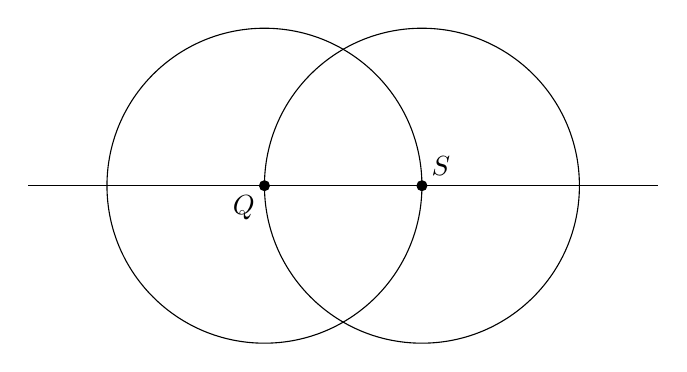
\begin{tikzpicture}
        % Círculos grandes
        \draw (1,0) circle(2cm);
        \draw (3,0) circle(2cm);
        % Línea horizontal
        \draw (-2,0)--(6,0);
        % Puntos
        \fill (1,0) circle(2pt) node[below left]{$Q$};
        \fill (3,0) circle(2pt) node[above right]{$S$};
    \end{tikzpicture}
        \caption{Prueba gráfica de que $S\subseteq S^c$.}
\end{figure}

\begin{definicion}
    Dado un conjunto de puntos del plano $S$, definimos recursivamente:
    \begin{equation*}
        S_0 = S, \quad S_{n+1} = S_n \qquad \forall n\in \mathbb{N}
    \end{equation*}
    Llamamos al conjunto:
    \begin{equation*}
        C(S) = \bigcup_{n\in \mathbb{N}}S_n
    \end{equation*}
    el conjunto de \underline{los puntos constructibles (con regla y compás) a partir de $S$}.
\end{definicion}

\begin{ejercicio}
    Construir a partir de tres puntos que no estén en la misma recta un cuarto punto que complete el paralelogramo.\\

    \noindent
    Para ello, primero necesitamos considerar la construcción de la mediatriz, con la que obtenemos el punto medio entre dos puntos $P$ y $Q$. Esta viene dada por la figura siguiente:
    \begin{figure}[H]
        \centering
        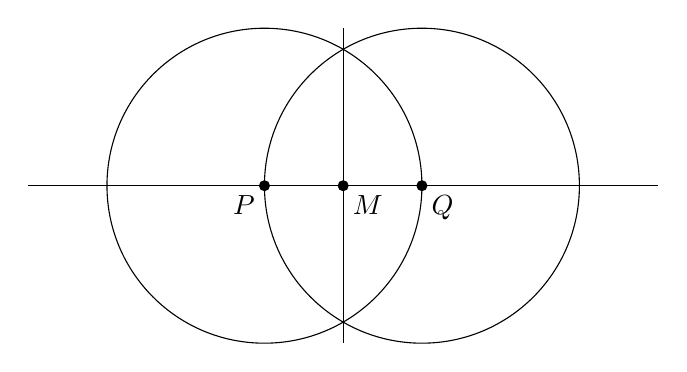
\begin{tikzpicture}
            \draw (-4, 0)--(4,0);
            \draw(0,2)--(0,-2);

            \draw (-1,0) circle(2cm);
            \draw (1,0) circle(2cm);

            \fill (-1,0) circle(2pt) node[below left]{$P$};
            \fill (1,0) circle(2pt) node[below right]{$Q$};
            \fill (0,0) circle(2pt) node[below right]{$M$};
        \end{tikzpicture}
    \end{figure}
    Una vez sabemos como realizar el punto medio de dos puntos dados, supongamos que tenemos 3 puntos: $P$, $Q$ y $R$ no alineados y que queremos trazar el cuarto punto que completa el paralelogramo. En dicha situación, trazamos las rectas $PQ$ y $PR$, así como la recta $RQ$. Trazamos el punto medio $M$ entre los puntos $R$ y $Q$, que hemos visto anteriormente cómo hacerlo. Ahora, trazamos la recta $PM$ y la circunferencia con centro $M$ y radio hasta $P$. El punto de intersección de estos dos últimos elementos geométricos nos dan el punto $T$ que completa el paralelogramo.
    \begin{figure}[H]
        \centering
        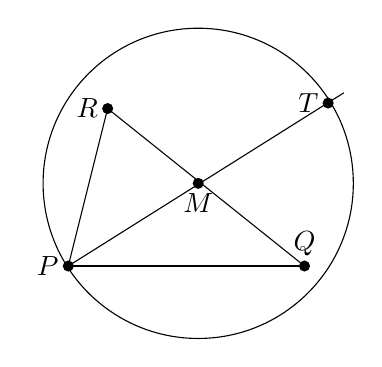
\begin{tikzpicture}
            \draw(-1,0) -- (2,0);
            \draw(-0.5,2) -- (-1,0);
            \draw(-0.5,2)--(2,0);
            \draw(-1,0) -- (2.5,2.2);
            \draw(0.65, 1.05) circle(1.97cm);

            \fill (-1,0) circle(2pt) node[left]{$P$};
            \fill (2,0) circle(2pt) node[above]{$Q$};
            \fill (-0.5,2) circle(2pt) node[left]{$R$};
            \fill (0.65,1.05) circle(2pt) node[below]{$M$};
            \fill (2.3,2.07) circle(2pt) node[left]{$T$};
        \end{tikzpicture}
    \end{figure}
\end{ejercicio}

\begin{lema}
    Sean $P,Q,R$ puntos del plano con $P$ y $Q$ distintos, se puede construir con regla y compás a partir de ellos un punto $T$  tal que las rectas $PQ$ y $RT$ son perpendiculares.
    \begin{proof}
        Distinguimos casos en función de la posición relativa de $P$, $Q$ y $R$:
        \begin{description}
            \item [Suponiendo que $R$ está en la recta $PQ$:] Trazamos la recta $PQ$ y la circunferencia con centro $R$ y que pasa por $Q$ (si $R=Q$, la que pasa por $P$), que nos da un punto intersección en $PQ$: $S$. Trazamos las circunferencias con centro $Q$ y radio hasta $S$, y centro $S$ y radio hasta $Q$. Estas dos circunferencias se cortan en dos puntos: $T$ y $T'$. Uniéndolos, obtenemos lo buscado.
            \begin{figure}[H] % // TODO: Cambiar dibujo
                \centering
                    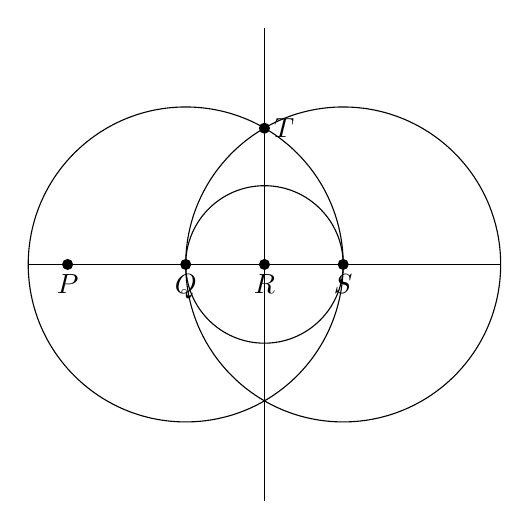
\begin{tikzpicture}

                    % Círculos grandes
                    \draw (1,0) circle(2cm);
                    \draw (3,0) circle(2cm);

                    % Círculo pequeño en el centro
                    \draw (2,0) circle(1cm);

                    % Línea horizontal
                    \draw (-1,0)--(5,0);

                    % Línea vertical
                    \draw (2,-3)--(2,3);

                    % Puntos
                    \fill (-0.5,0) circle(2pt) node[below]{$P$};
                    \fill (1,0) circle(2pt) node[below]{$Q$};
                    \fill (2,0) circle(2pt) node[below]{$R$};
                    \fill (3,0) circle(2pt) node[below]{$S$};
                    \fill (2,1.73) circle(2pt) node[right]{$T$};
                    \end{tikzpicture}
            \end{figure}
            \item [Suponiendo que $R$ no está en la recta $PQ$:]
                Trazamos la recta $PQ$ así como la circunferencia de centro $R$ y radio hasta $Q$, que nos da un punto de intersección con $PQ$: $S$. Trazamos la circunferencia de centro $S$ y radio hasta $Q$, obteniendo un segundo punto de corte entre las dos circunferencias, $T$, que unimos con $R$ y obtenemos la situación pedida:
            \begin{figure}[H]
                \centering
                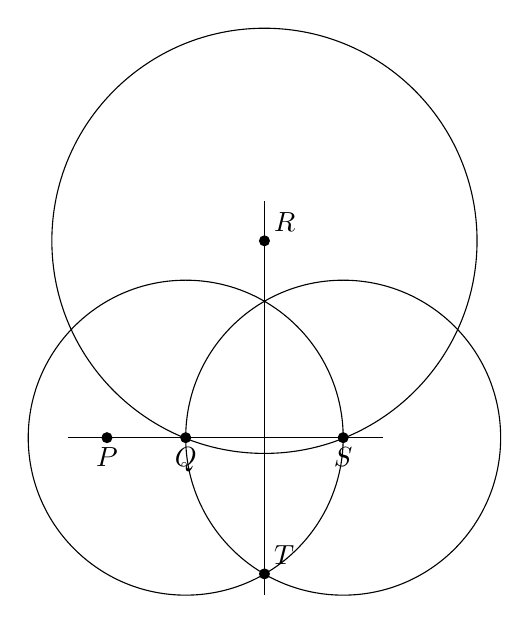
\begin{tikzpicture}
                    \draw(-2.5,0)--(1.5,0);
                    \draw(0,3)--(0,-2);

                    \draw(0,2.5) circle(2.7cm);
                    \draw(-1,0) circle(2cm);
                    \draw(1,0) circle(2cm);

                    \fill (-2,0) circle(2pt) node[below]{$P$};
                    \fill (-1,0) circle(2pt) node[below]{$Q$};
                    \fill (1,0) circle(2pt) node[below]{$S$};
                    \fill (0,2.5) circle(2pt) node[above right]{$R$};
                    \fill (0,-1.73) circle(2pt) node[above right]{$T$};
                \end{tikzpicture}
            \end{figure}
        \end{description}
    \end{proof}
\end{lema}
A partir del lema anterior, ya no será necesario recurrir a dichas construcciones cada vez que tengamos dos puntos $P$ y $Q$ que determinan una recta y queramos construir una recta perpendicular a ella que pase por un tercer punto $R$.

\begin{ejercicio}
    Dados dos puntos que determinan una recta $r$ y un punto $A$ no contenido en ella, construir el simétrico de $A$ con respecto de $r$.\\

    \noindent
    Sabemos ya por el lema anterior trazar una recta perpendicular a otra dada pasando por un punto, por lo que trazamos la recta perpendicular a $r$ que pasa por $A$. Al punto de intersección entre ambas rectas lo nombramos $O$, y trazando la circunferencia de centro $O$ y radio hasta $A$ obtenemos como intersección con la recta perpendicular a $r$ el punto $A'$, simétrico de $A$ respecto de $r$.

    \begin{figure}[H]
        \centering
        \begin{tikzpicture}
            \draw(0,2)--(0,-2);
            \draw(-2,0) -- (2,0);
            \draw(0,0) circle(1cm);
            \fill (1,0) circle(2pt) node[above right]{$A$};
            \fill (0,0) circle(2pt) node[below left]{$O$};
            \fill (-1,0) circle(2pt) node[above left]{$A'$};
            \fill (0.1,1.5) node[above right]{$r$};
        \end{tikzpicture}
    \end{figure}
\end{ejercicio}

\noindent
Si ahora elegimos dos puntos cualesquiera de $S$: $P$ y $Q$, podemos realizar la siguiente construcción:

\begin{figure}[H]
    \centering
    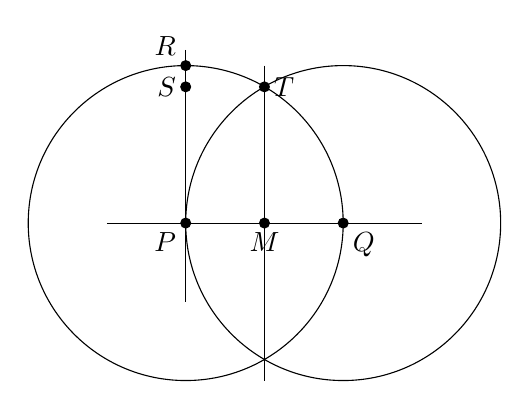
\begin{tikzpicture}
        \draw (0,0) circle(2cm);
        \draw (2,0) circle(2cm);
        \draw (1,2) -- (1,-2);
        \draw (0,2.2) -- (0,-1);
        \draw (-1,0) -- (3,0);
        \fill (0,0) circle(2pt) node[below left]{$P$};
        \fill (2,0) circle(2pt) node[below right]{$Q$};
        \fill (1,0) circle(2pt) node[below]{$M$};
        \fill (1,1.73) circle(2pt) node[right]{$T$};
        \fill (0,1.73) circle(2pt) node[left]{$S$};
        \fill (0,2) circle(2pt) node[above left]{$R$};
    \end{tikzpicture}
\end{figure}

Trazar las dos circunferencias que definen los puntos $P$ y $Q$, con lo que trazamos la mediatriz, la recta que se obtiene uniendo los puntos de intersección de las dos circunferencias. Nombramos a un punto de dicha intersección $T$. Trazamos la recta $PQ$ y obtenemos su intersección con la recta previamente trazada en el punto $M$. A continuación, completamos el cuadrilátero que definen los puntos $P$, $M$ y $T$ con el punto $S$, que nos permite considerar la recta $PS$. Si finalmente obtenemos la intersección de la recta $PS$ con la circunferencia de centro $P$ y radio hasta $Q$ obtenemos el punto $R$, que pertenece a la recta $PS$, perpendicular a la recta $PQ$ y el punto $R$ se encuentra a la misma distancia que $Q$ del punto $P$, corte de las dos rectas perpendiculares.

Hemos obtenido lo que consideraríamos un sistema de referencia ortonormal, y podemos renombrar a los puntos $P$, $Q$ y $R$ como $(0,0)$, $(1,0)$ y $(0,1)$, respectivamente. De esta forma, podemos ver el conjunto $C(S)$ de puntos constructibles a partir de $S$ como un subconjunto de $\mathbb{C}$. A partir de ahora, supondremos siempre que $S$ es un conjunto que contiene a los números $0$ y $1$.

La pregunta natural que surge al hacer esta observación es la de fijado un conjunto inicial $S\subseteq \mathbb{C}$, qué puntos de $\mathbb{C}$ son constructibles a partir de $S$. Es decir, obtener una descripción de $C(S)$.

\begin{observacion}
    Puesto que ahora suponemos que $0,1\in S$, es muy fácil ver que $i \in C(S)$, ya que podemos realizar la construcción anterior para $P = 0$, $Q= 1$ y tomar $R = i$, por lo que podemos usar que $i \in C(S)$.
\end{observacion}

\begin{lema}
    Dado $z=x+iy\in \mathbb{C}$, tenemos que:
    \begin{equation*}
        z\in C(S) \Longleftrightarrow x,y\in C(S)
    \end{equation*}
    \begin{proof}
        Por doble implicación:
        \begin{description}
            \item [$\Longrightarrow )$] Supuesto que $z\in C(S)$, vemos que podemos construir $x$ e $y$ de la siguiente forma:
                \begin{itemize}
                    \item Si $z\in \mathbb{R}$, tenemos ya construido $x=z$ y sabemos que $y=0\in C(S)$.
                    \item Si $Re(z) = 0$, sabemos que $x=0\in C(S)$ y tenemos el punto $z=iy$ que construiremos en el siguiente apartado.
                    \item En otro caso, podemos considerar la recta $01$ y trazar la recta perpendicular a ella que pasa por el punto $z$. Como la intersección de las dos rectas obtenemos el punto $x$. Ahora, si consideramos la recta $0i$ y trazamos la recta perpendicular a ella que pasa por el punto $z$, obtenemos el punto $iy$. Para obtener $y$, lo que haremos será considerar la intersección de la recta $01$ con la circunferencia de centro $0$ y radio hasta $iy$:
                        \begin{figure}[H]
                            \centering
                            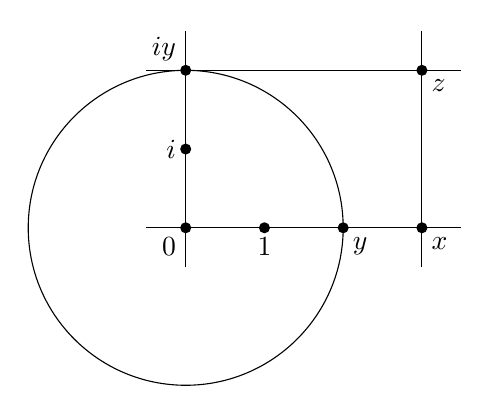
\begin{tikzpicture}
                                \draw(-0.5,0) -- (3.5,0);
                                \draw(0,-0.5) -- (0,2.5);
                                \draw(3,2.5) -- (3,-0.5);
                                \draw(-0.5,2) -- (3.5,2);
                                \draw(0,0) circle(2cm);
                                \fill(0,0) circle(2pt) node[below left]{$0$};
                                \fill(1,0) circle(2pt) node[below]{$1$};
                                \fill(0,1) circle(2pt) node[left]{$i$};
                                \fill(3,2) circle(2pt) node[below right]{$z$};
                                \fill(3,0) circle(2pt) node[below right]{$x$};
                                \fill(0,2) circle(2pt) node[above left]{$iy$};
                                \fill(2,0) circle(2pt) node[below right]{$y$};
                            \end{tikzpicture}
                        \end{figure}
                \end{itemize}
            \item [$\Longleftarrow )$] Supuesto que $x,y\in C(S)$, lo que haremos será considerar la recta perpendicular a la recta $0x$ que pasa por el punto $x$, obteniendo la recta $r$. Posteriormente, consideraremos como $iy$ la intersección de la recta $0i$ con la circunferencia de centro $0$ y radio hasta $y$. Posteriormente, trazamos la recta perpendicular a $0i$ que pasa por $iy$, y obtenemos como $z$ la intersección de esta última recta con la recta $r$.
                \begin{figure}[H]
                    \centering
                    \begin{tikzpicture}
                        \draw (-0.5,0) -- (3.5,0);
                        \draw (0,-0.5) -- (0,3.5);
                        \draw (2,-0.5) -- (2,3.5);
                        \draw (-0.5,3) -- (2.5,3);
                        \draw (0,0) circle(3cm);
                        \fill(0,0) circle(2pt) node[below left]{$0$};
                        \fill(0,1) circle(2pt) node[left]{$i$};
                        \fill(2,0) circle(2pt) node[below left]{$x$};
                        \fill(3,0) circle(2pt) node[below left]{$y$};
                        \fill(2,3) circle(2pt) node[below left]{$z$};
                        \fill(0,3) circle(2pt) node[below left]{$iy$};
                        \fill(2,1) node[left]{$r$};
                    \end{tikzpicture}
                \end{figure}
        \end{description}
    \end{proof}
\end{lema}
